\chapter{Planificación}

\section {Fases y entregas}
\subsection {Fases}

Este proyecto estará compuesto por seis fases, cobrando un gran peso en tiempo tres de ellas, la Análisis y diseño, la Implementación ( aunque se parta de una base de código iniciada con anterioridad) y la de pruebas, todas las fases serán las siguientes:

\begin{itemize}
  \item Fase 1: Especificaciones del proyecto.
  \item Fase 2: Planificación.
  \item Fase 3: Análisis y diseño.
  \item Fase 4: Desarrollo.
\end{itemize}

\subsection {Lista de actividades}
A continuación se muestra las actividades a desarrollar en cada fase. Como se puede observar, debido a nuestra orientación DevOps, una vez que en las primeras fases hemos conseguido una idea relativamente definida, pero no final, sobre la que podemos sentar las bases del proyecto , comenzamos una cuarta fase, en la cual se llevan en paralelo y de forma incremental varias tareas, como son la implementación, la documentación y las pruebas, pruebas que representan la especificación.

\begin{itemize}
  \item Fase 1: Especificaciones del proyecto.
    \begin{enumerate}
      \item Determinación objetivos.
      \item Determinación requisitos.
    \end{enumerate}
  \item Fase 2: Planificación.
    \begin{enumerate}
      \item Lista de actividades
      \item Entrevistas
      \item Presupuesto
    \end{enumerate}
  \item Fase 3: Análisis y diseño.
    \begin{enumerate}
      \item Análisis de requisitos
      \item Diagramas
      \item Metodología de desarrollo.
      \item Descripción estructural
    \end{enumerate}
  \item Fase 4: Desarrollo.
    \begin{itemize}
       \item \textbf{Implementación:} 
       \begin{itemize}
         \item  Infraestructura.
         \item  Base de datos.
         \item  Backend.
         \item  Fronted.
       \end{itemize}
       \item \textbf{Pruebas:} 
       \begin{itemize}
        \item  \gls{Test unitarios}.
        \item  \gls{Test de cobertura}.
        \item  \gls{Integracion continua}.
        \item  \gls{Despliegue continuo}.
       \end{itemize}
       \item \textbf{Documentación:} 
       \begin{itemize}
        \item  API/BackEnd.
        \item  FrontEnd.
        \item  Proyecto.
       \end{itemize}
    \end{itemize}
\end{itemize}

En la siguiente imagen \ref{fig:gantt}, se muestra un diagrama de Gantt con la planificación seguida.

\begin{figure}
  \begin{center}
    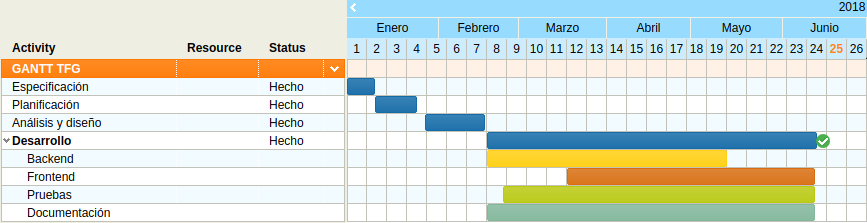
\includegraphics[width=\textwidth]{imagenes/gantt.png}
    \caption{Diagrama de Gantt}
    \label{fig:gantt}
  \end{center}
\end{figure}



\section {Entrevistas}
Para poder alcanzar una interfaz cómoda y de calidad, se ha realizado una serie de preguntas un \gls{test A/B} a varios usuarios, de forma que usando el feedback proporcionado se han tomado las decisiones para la forma en la que se introducen y se muestran los datos.

\section {Presupuestos}

Para este proyecto se ha utilizado software libre y versiones gratuitas de ciertas plataformas como Auth0, TravisCI, GitHub, GreenKeeper, SonnarQube, mLab, PaperTrail y Heroku entre otras. Por ello el coste en licencias en infraestructura de desarrollo es nulo. Cabe destacar que se han realizado despliegues en Google Cloud, que aunque se ha realizado haciendo uso de créditos gratuitos, si que conllevaría un gasto si se optara por mantener la aplicación en dicha plataforma.
En caso de querer realizar un despliegue permanente mencionado anteriormente y  suponiendo 7000 usuarios mensuales activos, el precio de la autenticación seguiría siendo gratuito aunque
por otro lado está el coste de la infraestructura. Debido a que la mayor parte de la computación
se hace en el lado del cliente, no se requiere un hardware de gran potencia, por ello optamos por
una máquina con 3.75Gb de RAM, 200GB de almacenamiento, 1 CPU y 456 horas de uso real al mes, lo cual, alojado en Google Cloud, nos costaría un total de 22,11\euro  al mes. Al margen de los costes de infraestructura y licencia, también se debe tener en cuenta el precio del desarrollo, con un tiempo  de 400 horas de trabajo y suponiendo un salario de 12\euro  la hora, habría que valorar en 4800\euro .
